\documentclass{article}
\usepackage[utf8]{inputenc}
\usepackage{fullpage}
\usepackage{amsmath}
\usepackage{mathtools}
\usepackage{enumerate}
\usepackage[parfill]{parskip} % New line instead of indentation for new paragraphs.
\usepackage{graphicx}
\usepackage{listings} % Allows for math inside verbatim
\usepackage{url}
\lstset{
  basicstyle=\ttfamily,
  mathescape
}
\graphicspath{{figures/}}

\title{EDA387: Computer Networks - Lab 2.2}
\author{Mats Högberg}
\date{\today}

\begin{document}

\maketitle

\section*{Mutual exclusion on a lollipop}

This problem can be solved by using fair composition of two algorithms: Spanning Tree Construction and Mutual Exclusion for Tree Structures, both of which are described in the course book. The idea is that each processor runs both algorithms in alternation, first one step of the Spanning Tree algorithm, then one step of the Mutual Exclusion algorithm, then one step of the Spanning Tree algorithm, and so on. The Mutual Exclusion algorithm will use the output of the Spanning Tree algorithm to construct a graph on which it can operate. Once the Spanning Tree algorithm has stabilized, the graph on which the Mutual Exclusion algorithm operates will be a spanning tree, which will allow the Mutual Exclusion algorithm to stabilize as well.

The Spanning Tree Construction algorithm stabilizes in $\Delta + 4 \hat{k} \Delta$ rounds, where $\Delta$ is the maximum number of links adjacent to any processor and $\hat{k}$ is the largest distance from the root processor to any other processor. In our graph we have that $\Delta = m$, and if we assume that the processor corresponding to node $v_m$ in the $(m,n)$-lollipop graph is the root, we have that $\hat{k} = n$. This means that the Spanning Tree Construction algorithm will stabilize in $m + 4nm \in O(nm)$ rounds. This algorithm requires registers with a size of at least $O(\log(\hat{k})) = O(\log(n))$, which is okay in our case.

Given the output from the Spanning Tree Construction algorithm we can construct the tree needed by the Mutual Exclusion for Tree Structures algorithm. For processor $p_i$ this is done by setting the processor $p_j$ where $r_{i,j} = 1$ as parent, and all processors $p_k$ where $r_{k, i} = 1$ as children. We will end up with a tree that looks like the one depicted in figure \ref{fig:tree}. When forming a ring from this tree, processor $v_m$ will act as $m$ processors, processors $v_1, \ldots, v_{m-1}$ and $u_n$ will each act as a single processor, and processors $u_1, \ldots, u_{n-1}$ will each act as two processors. In total, our ring will have $2(m + n - 1) \in O(m+n)$ virtual processors, and each virtual processor will have 2 registers, one local and one non-local. Our ring must be able to hold thus $O(2(m+n)) = O(m+n)$ different values, which can be done with registers of size $O(\log(m+n))$. The time until stabilization for the Mutual Exclusion algorithm will be $O((m+n)^2)$, given that the Spanning Tree Construction algorithm has already stabilized, and combining this with the time until stabilization for the Spanning Tree Construction algorithm we have that our entire system will stabilize in $O(nm + (m+n)^2) = O((m+n)^2)$ rounds.

\begin{figure}
    \centering
    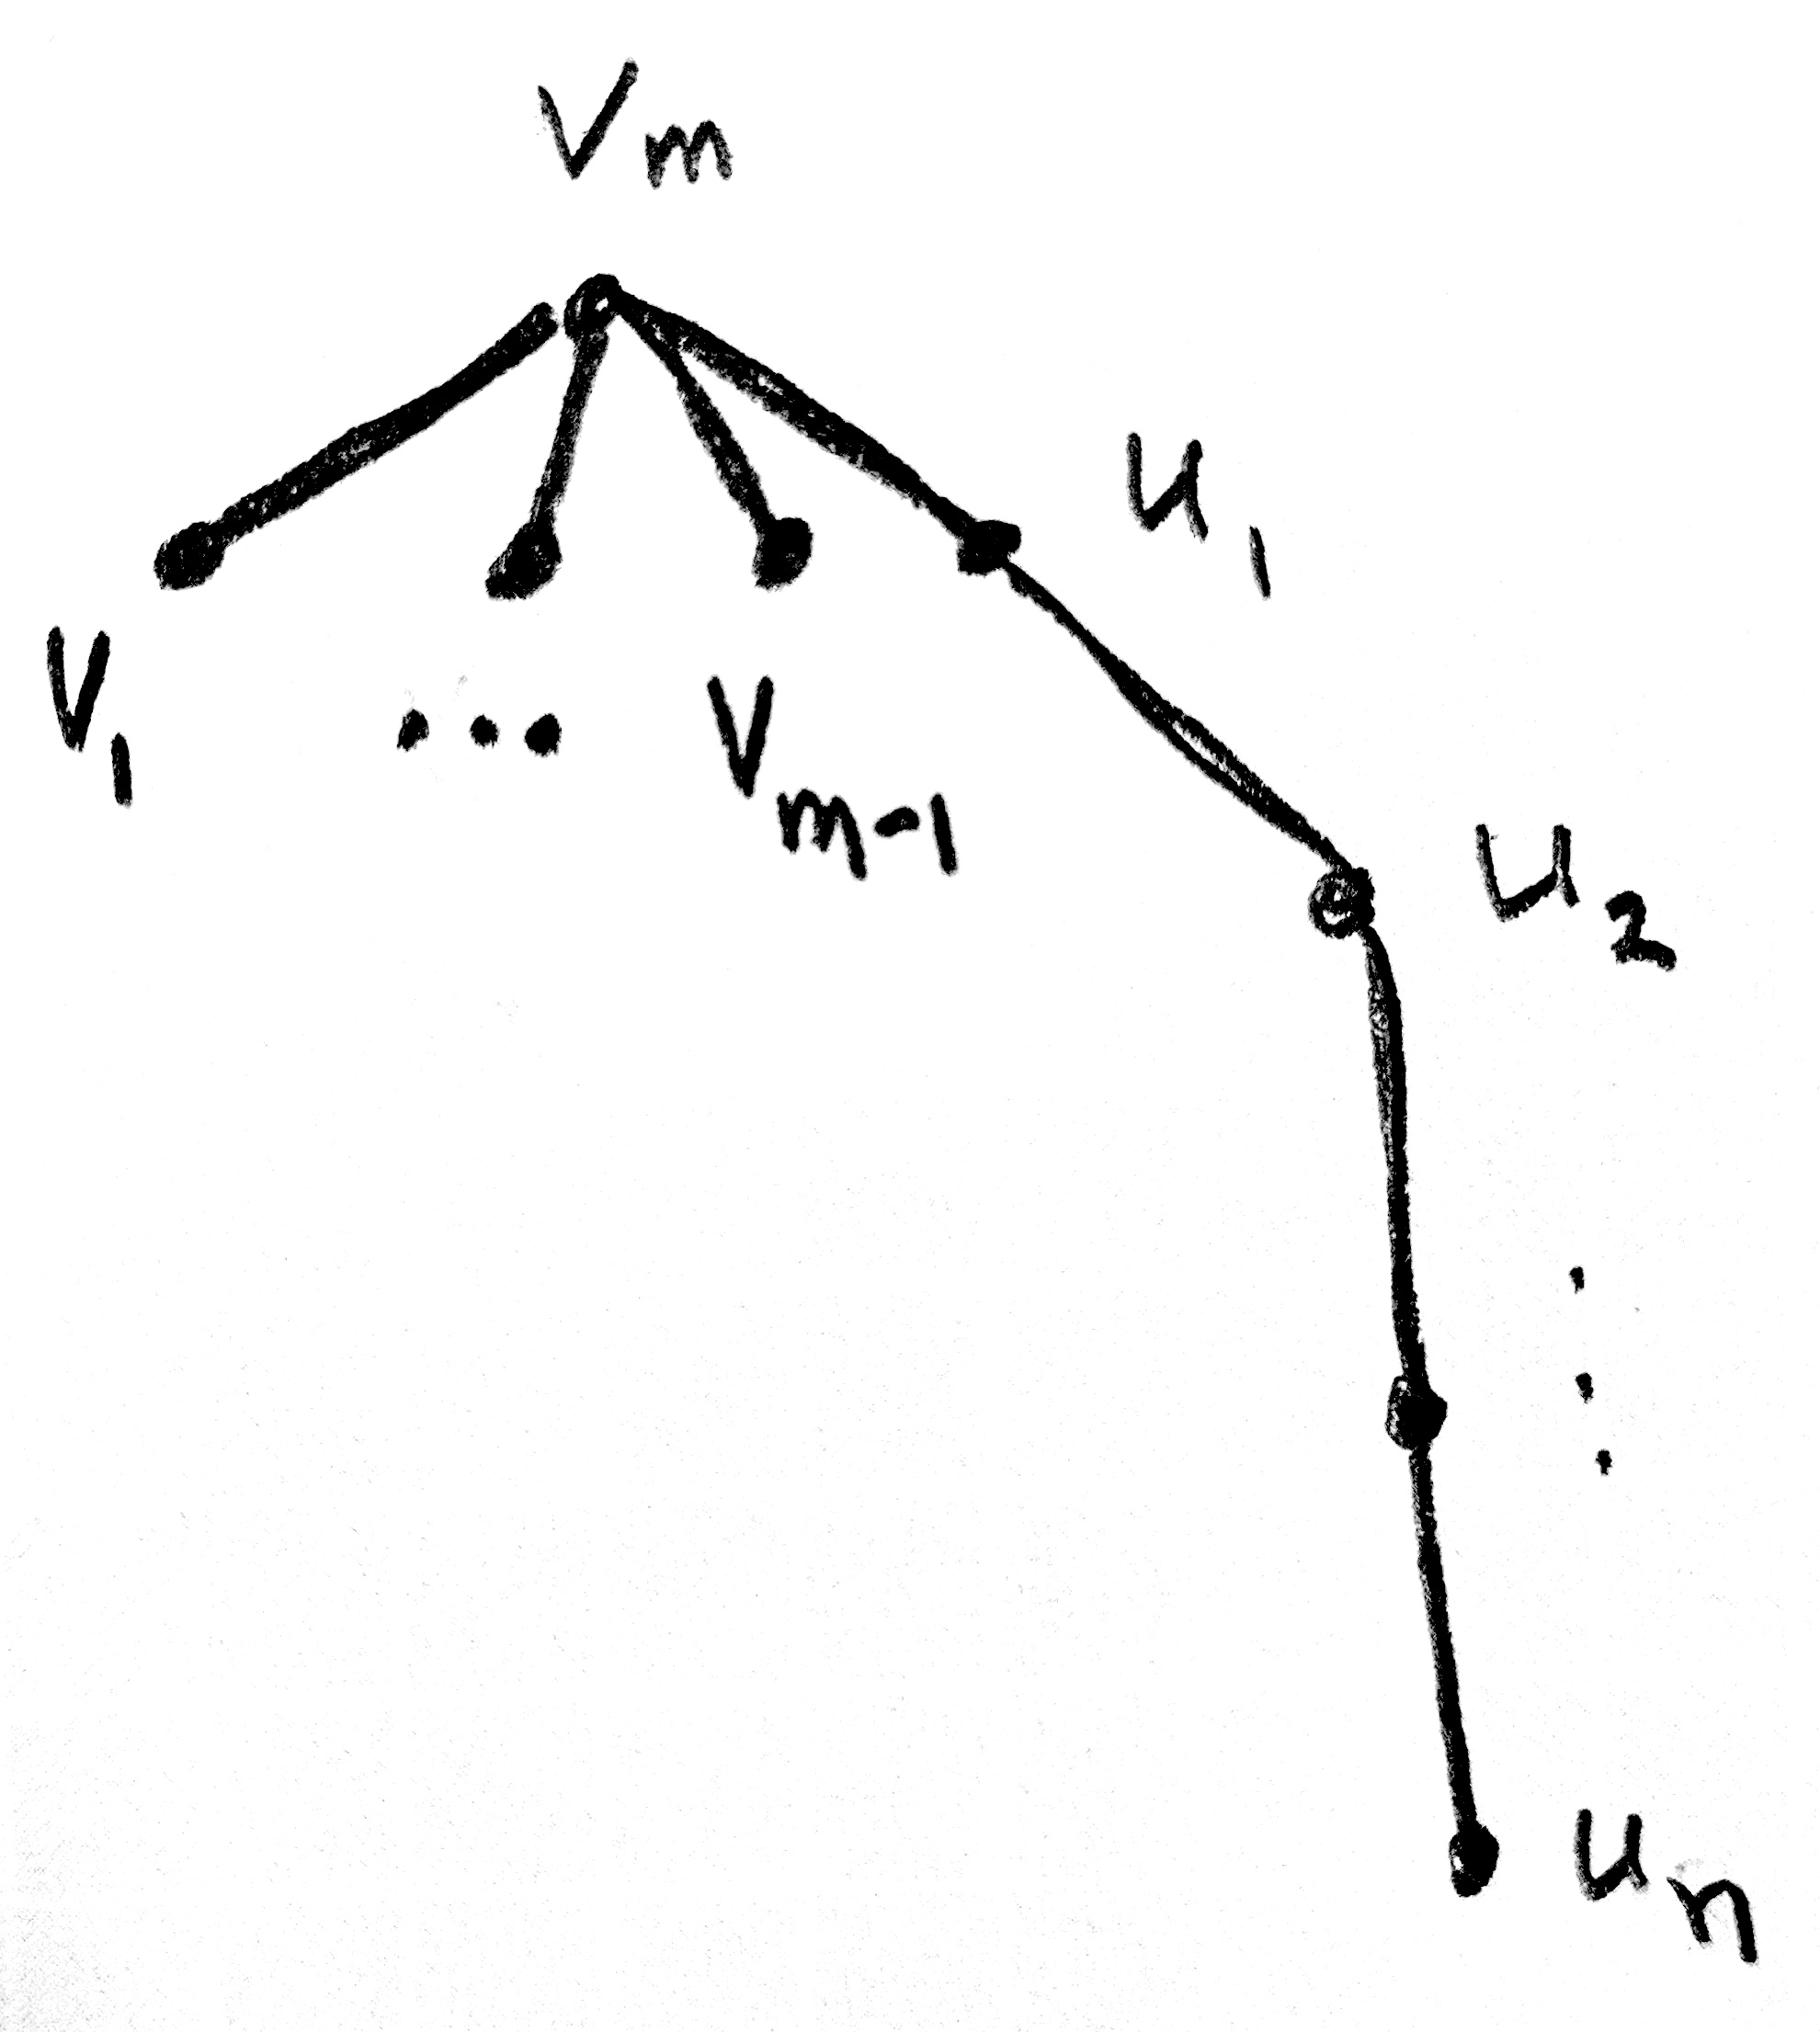
\includegraphics[width=\linewidth]{tree}
    \caption{The tree constructed by the Spanning Tree Construction algorithm.}
    \label{fig:tree}
\end{figure}

\end{document}
